\chapter{Resultados e discussões}\label{Resultados}

\section{Resultados}

Para a apresentação dos resultados, foram escolhidos escolhido dois pontos na cidade de Pelotas, o ShoppingPelotas \cite{shoppingpelotas} e uma residência.

O ShoppingPelotas é um estabelecimento com as características perfeitas para demonstrar o resultado, pois tem uma grande área de cobertura do prédio e de estacionamento com mais de 100 vagas.

A residencia é do autor do trabalho, foi escolhida um pouco por curiosidade para saber os resultados na residencia que moro, porem esta é uma residencia com características comuns tem uma grande área de telhado não utilizado exatamente como a maioria dos prédios e casas do mundo.

\subsection{Resultados Shopping Pelotas}

Primeiro, é necessário verificar a área disponível do estabelecimento. Utilizando a ferramenta do Google Earth \cite{Earth} é possível encontrar e medir a área útil de um local no globo. A Figura \ref{fig:shopping_1} mostra a área da cobertura shopping, a Figura \ref{fig:shopping_2} mostra a área de estacionamento do shopping.

\begin{figure}[H]
    \centering
    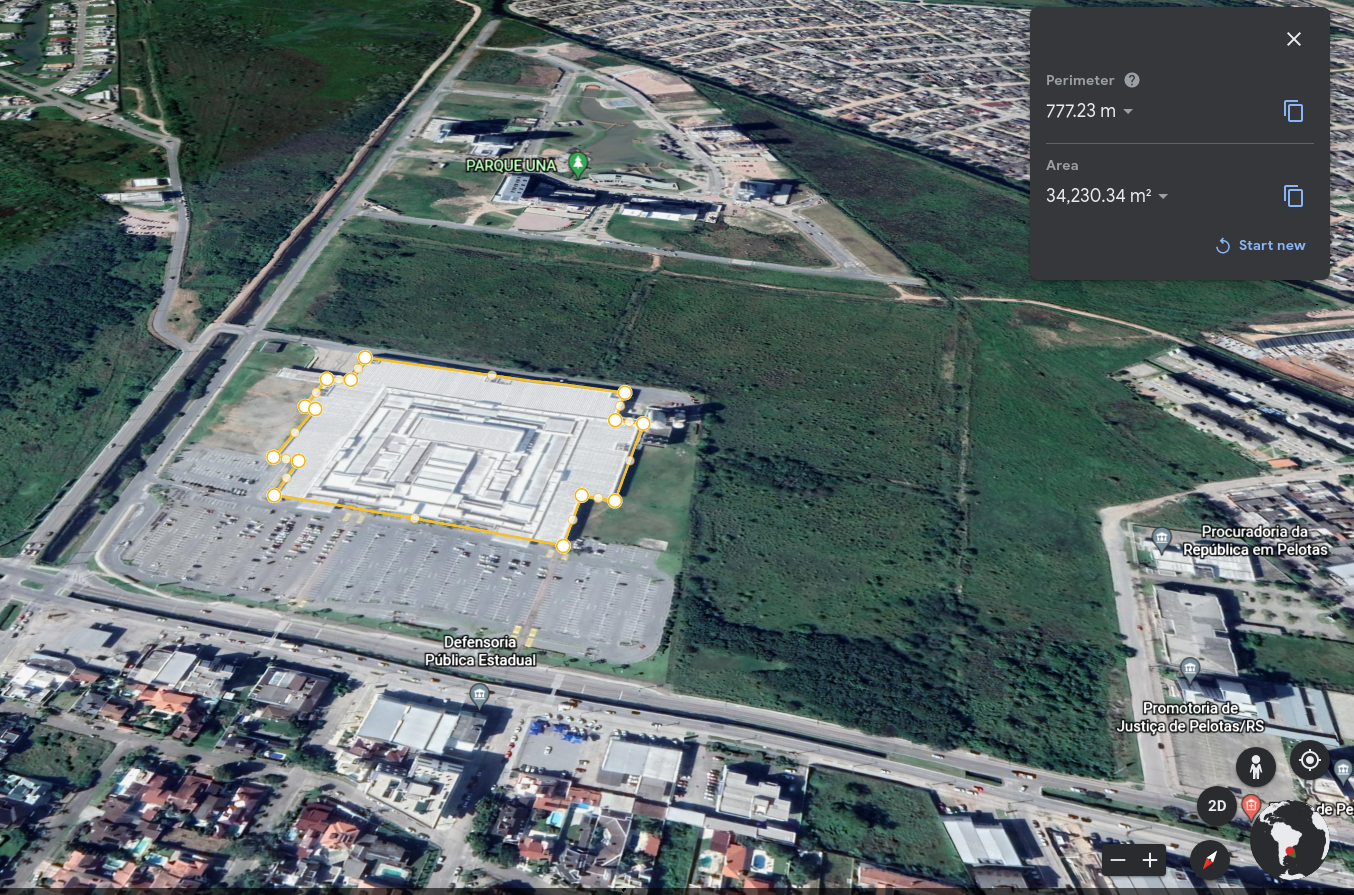
\includegraphics[width=1\textwidth]{./Figuras/shopping_1.png}
    \caption{Área da cobertura Shopping.}
   \label{fig:shopping_1}
\end{figure}

\begin{figure}[H]
    \centering
    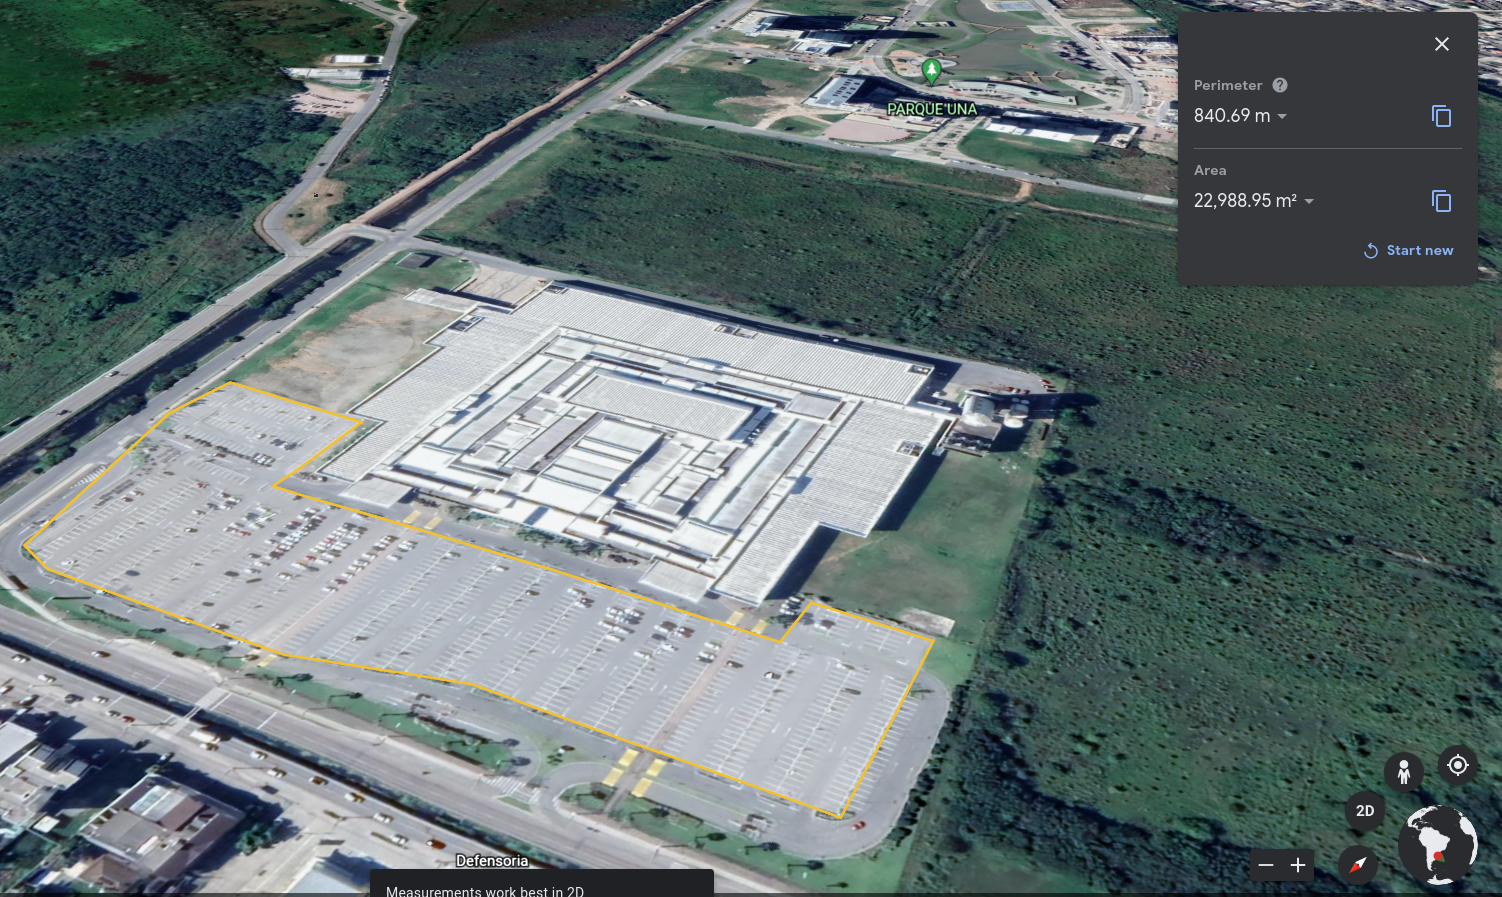
\includegraphics[width=1\textwidth]{./Figuras/shopping_2.png}
    \caption{Área do estacionamento Shopping.}
   \label{fig:shopping_2}
\end{figure}

\newpage
Como é possível ver pelas Figuras \ref{fig:shopping_1} e \ref{fig:shopping_2}, o ShoppingPelotas tem uma área total de cerca de 57 mil m². A partir destes dados, é possível determinar a capacidade de produção de energia e simular algumas situações.

\subsection{Produção de energia total anual do Shopping Pelotas}

Usando o valor total da área do shopping, podemos determinar a capacidade máxima aproximada de produção de energia anual. Para isto no aplicativo é selecionado ``Área total'' como modelo de entrada, alterado o valor da ``Área total utilizada'' para 57000 e o ``Consumo de energia mensal'' para 175000 um valor estimado de consumo do estabelecimento, todos os outros valores foi deixado o padrão do sistema de entradas, assim temos as entradas da Figura \ref{fig:shopping_3}, obtém-se os resultados na Figura \ref{fig:shopping_4}.

\begin{figure}[H]
    \centering
    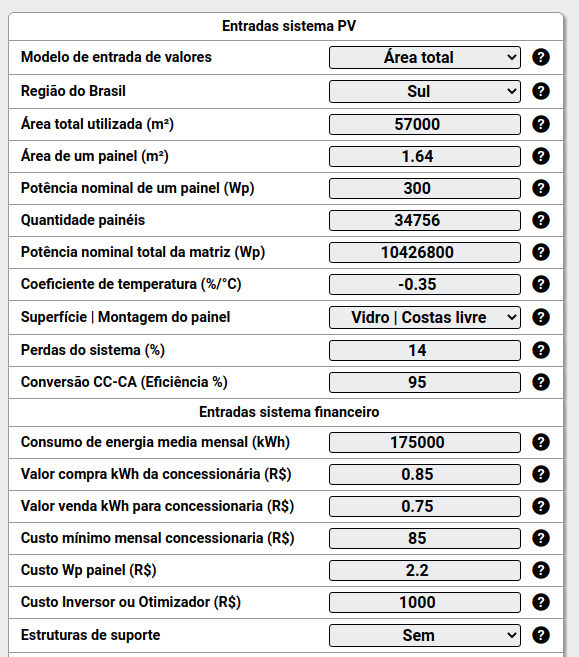
\includegraphics[width=0.8\textwidth]{./Figuras/shopping_3.png}
    \caption{Shopping Pelotas produção de energia total anual - entrada.}
   \label{fig:shopping_3}
\end{figure}

\begin{figure}[H]
    \centering
    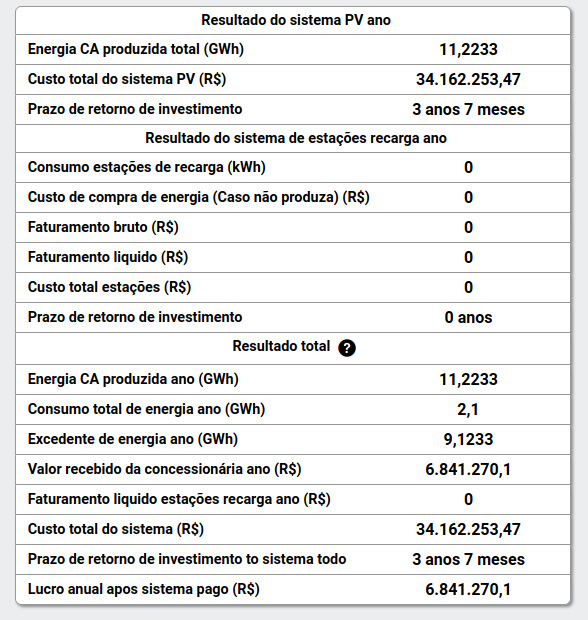
\includegraphics[width=0.9\textwidth]{./Figuras/shopping_4.png}
    \caption{Shopping Pelotas produção de energia total anual resultado.}
   \label{fig:shopping_4}
\end{figure}

Desta forma, é possível ver que o consumo estimado do shopping é de 2,1 GWh ano e a capacidade máxima de produção de energia, utilizando painéis de 300 $W_{p}$, é de 11,2233 GWh. Portanto, o shopping é capaz de produzir bem mais energia do que consome, o que permite utilizar o Shopping como estação de recarga e cogeração de energia sem ficar dependente de energia da rede.

\newpage
\subsection{Shopping Pelotas utilizado com estação de recarga e cogeração de energia}

Para essa estimativa, foi utilizada a área de 30.000 m², como área útil do teto do estabelecimento. Para isto no aplicativo é selecionado ``Área total'' como modelo de entrada, alterado o valor da ``Área total utilizada'' para 30000 e o ``Consumo de energia mensal'' para 175000 um valor estimado de consumo do estabelecimento, foi selecionada ``Laje/telhado'' em estruturas de suporte e a quantidade de estruturas 9150 (cada estrutura suporta dois painéis), foi selecionada ``Com'' estações de recarga VE e foi adicionado 20 estações ultrarrápidas e 66 rápidas, todos os outros valores foi deixado o padrão do sistema de entradas, conforme pode ser observado nas Figuras \ref{fig:shopping_5_1} e \ref{fig:shopping_5_2}.

\begin{figure}[H]
    \centering
    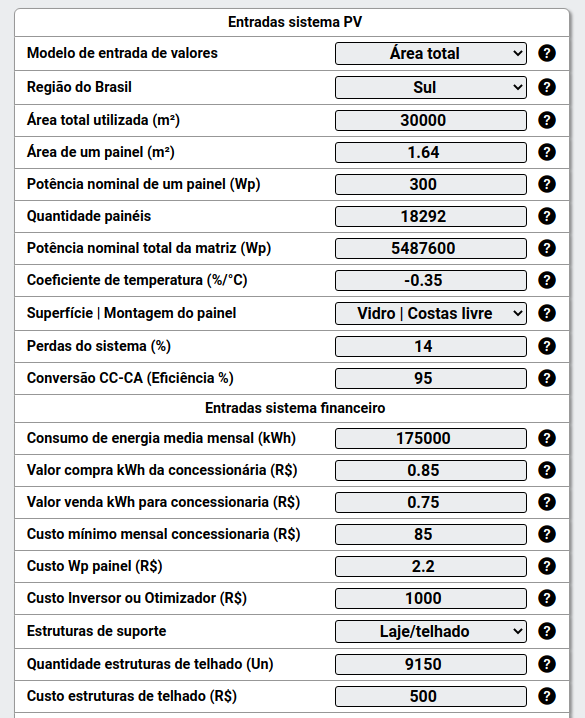
\includegraphics[width=0.75\textwidth]{./Figuras/shopping_5_1.png}
    \caption{Entradas da estimativa do shopping como estação de recarga e cogeração de energia.}
   \label{fig:shopping_5_1}
\end{figure}

\begin{figure}[H]
    \centering
    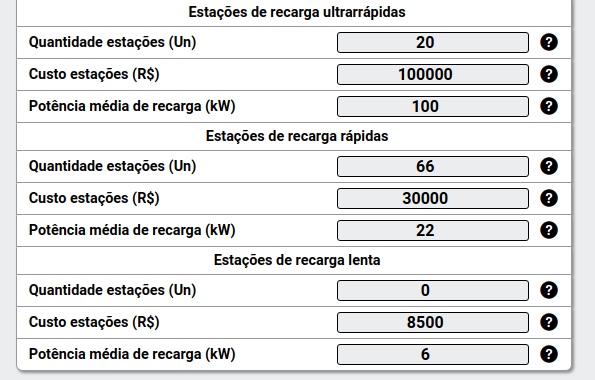
\includegraphics[width=1\textwidth]{./Figuras/shopping_5_2.png}
    \caption{Entradas da estimativa do shopping como estação de recarga e cogeração de energia.}
   \label{fig:shopping_5_2}
\end{figure}

Os resultados são mostrados na Figura \ref{fig:shopping_6}. No resultados do sistema PV temos um produção de energia estimada de 5,9 GWh e um custo de mais de 22 milhões de reais e um prazo de retorno do investimento de 4 anos e 6 meses, este prazo é estimado que toda energia produzida foi consumida pelo estabelecimento.

No resultado do sistema de estação de recarga as estações consumirão 3,78 GWh de energia, caso toda esta energia viesse da rede o faturamento liquido anual seria de 567 mil reais, com este faturamento o retorno do investimento das estações é estimado em 7 anos e 1 mês.

Quando analisamos o sistema como um todo, vemos que a produção de energia é maior que o consumo o que garante o melhor lucro e retorno no investimento, pois toda energia produzida que não foi usada pelo estabelecimento foi vendida nas estações de recarga, e o excedente de energia foi vendido para concessionária e como este valor é alto o suficiente para pagar o custo mínimo de conexão com a rede a venda do excedente só gera lucro, com isso prazo de retorno do sistema é de 4 anos e 9 meses, quando comparamos com o tempo de retorno somente das estações de recarga vemos que a cogeração de energia produz prazos de retornos bem mais atrativos, o sistema tem uma expectativa de vida longa em torno de 20 a 25 anos após o período de retorno no investimento gera um lucro anual liquido de 3,8 milhões de reais, o que resulta em uma estimativa de lucro de mais de 55 milhões em 25 anos o que é um retorno de mais de 200\% no valor investido total.

\begin{figure}[H]
    \centering
    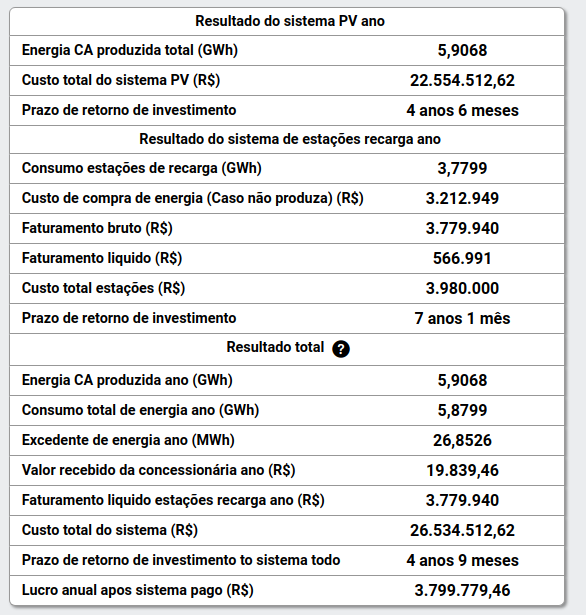
\includegraphics[width=1\textwidth]{./Figuras/shopping_6.png}
    \caption{Resultado da estimativa do shopping como estação de recarga e cogeração de energia.}
   \label{fig:shopping_6}
\end{figure}

No resultado mostrado na Figura \ref{fig:shopping_6}, foi estimado que existe trafego de veículos elétricos utilizando as estações.  Porém, no início da implementação do sistema pode não ter trafego, assim, basta apenas mudar a entrada ``“Média de Horas de utilização por dia'' para zero.   Dessa forma,  obtém-se obtém o resultado da Figura 75

\begin{figure}[H]
    \centering
    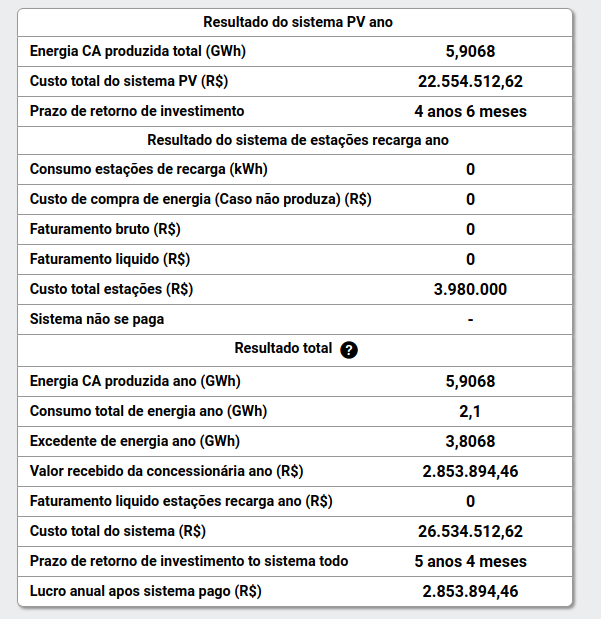
\includegraphics[width=0.9\textwidth]{./Figuras/shopping_7.png}
    \caption{Resultado da estimativa do shopping como estação de recarga e cogeração de energia, trafego veículos elétricos zero.}
   \label{fig:shopping_7}
\end{figure}

Como se pode observar, por meio dos resultados, o sistema acaba se pagando e, após 5 anos e 4 meses, só produz lucro. Na medida em que o sistema de recarga começa a ser usado, o lucro anual aumenta. Caso a utilização das estações gere um déficit de produção de energia, é possível expandir a área de estacionamento para a produção de energia e assim suprir a demanda sem causar dependência da rede elétrica.

\newpage
\subsection{Resultados para uma residência}

Para essa estimativa, foi utilizada uma residência na cidade de Pelotas, conforme mostrado na Figura \ref{fig:casa_minha}, com uma área de telhado de cerca de de 40m², esta residência se encontra no sul do Brasil e tem grande parte do telhado voltado para o norte este recebe energia do sol diretamente em quase todo período do dia.

\begin{figure}[H]
    \centering
    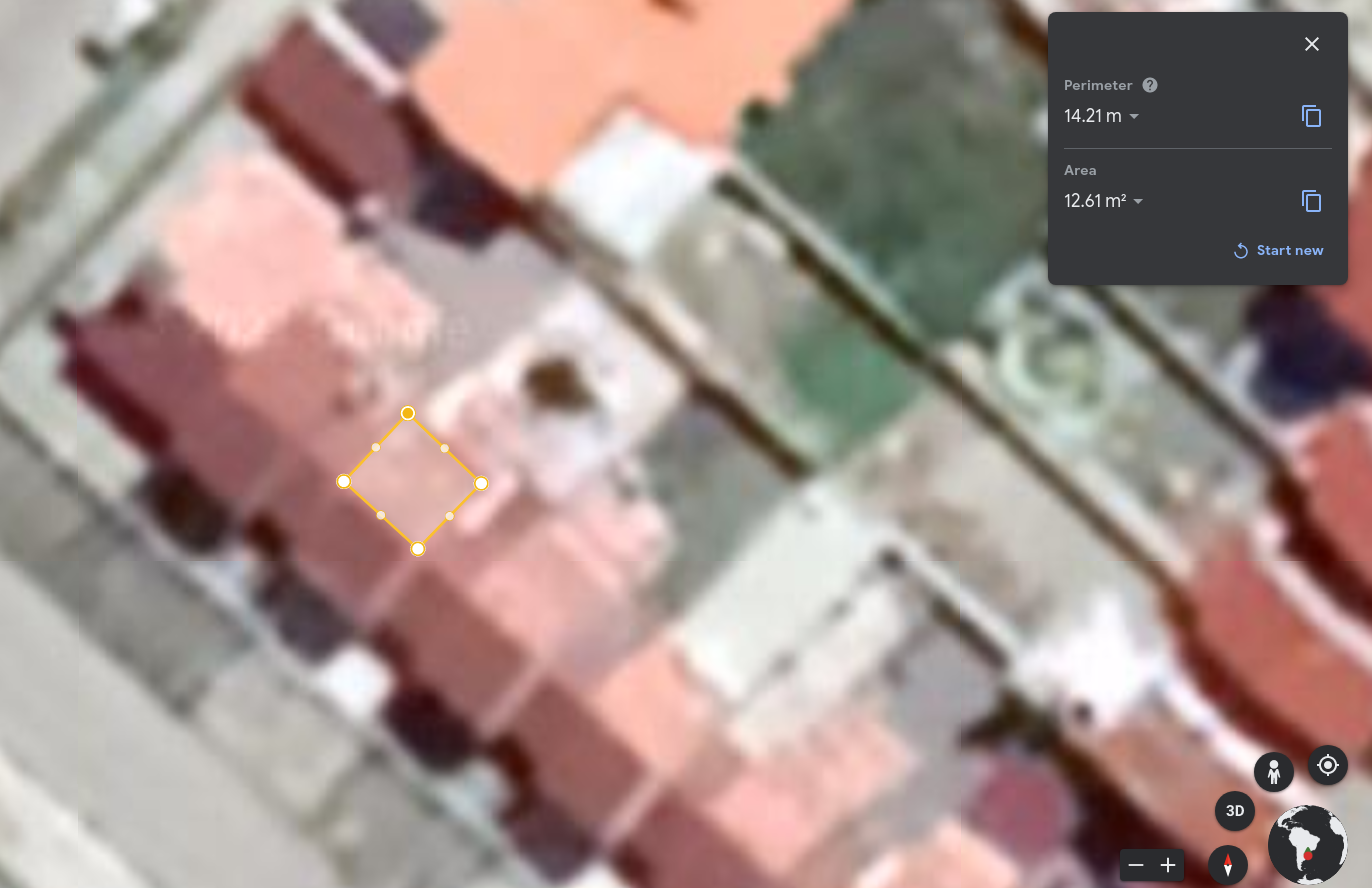
\includegraphics[width=0.8\textwidth]{./Figuras/casa_minha.png}
    \caption{Residência com telhado de 40 m² na cidade de Pelotas.}
   \label{fig:casa_minha}
\end{figure}

No aplicativo é selecionado ``Área total'' como modelo de entrada, alterado o valor da ``Área total utilizada'' para 14 e o ``Consumo de energia mensal'' para 175 um valor estimado de consumo do estabelecimento,  foi selecionada ``Laje/telhado'' em estruturas de suporte e a quantidade de estruturas 4 (cada estrutura suporta dois painéis), todos os outros valores foi deixado o padrão do sistema de entradas, conforme pode ser observado nas Figura \ref{fig:casa_minha_1}.

\begin{figure}[H]
    \centering
    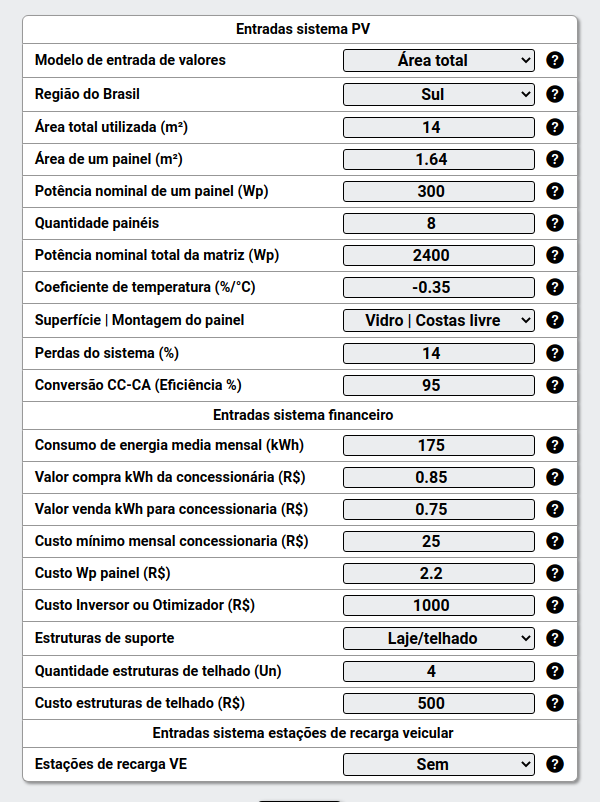
\includegraphics[width=0.8\textwidth]{./Figuras/casa_minha_1.png}
    \caption{Entradas para uma residência com telhado de 40 m² na cidade de Pelotas.}
   \label{fig:casa_minha_1}
\end{figure}

Na Figura \ref{fig:casa_minha_1_2}, tem-se o resultado, como toda a energia produzida é consumida e a energia excedente é vendida para a concessionária é o suficiente para pagar a taxa mínima de conexão com a rede assim o prazo de retorno final é de 4 anos e 8 meses.

\begin{figure}[H]
    \centering
    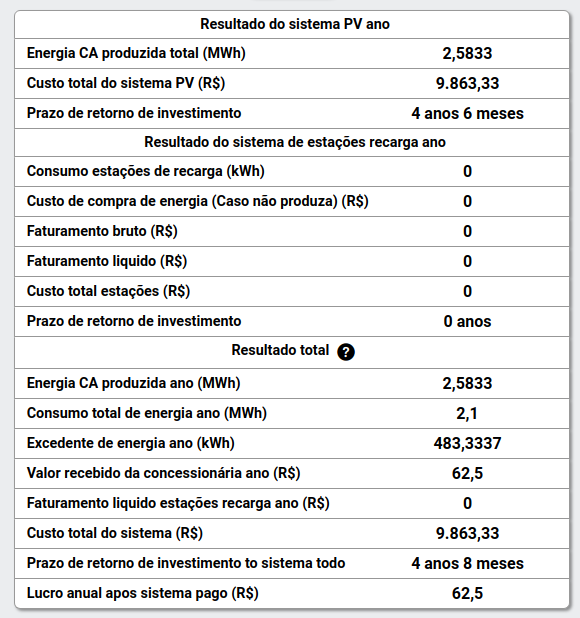
\includegraphics[width=0.875\textwidth]{./Figuras/casa_minha_1_2.png}
    \caption{Resultado para uma residência com telhado de 40 m² na cidade de Pelotas.}
   \label{fig:casa_minha_1_2}
\end{figure}

Admitindo que essa residência tenha um veículo elétrico e que este veículo percorre cerca de 250 km por semana, e por isso consome 33,25kWh, em média por semana ou 1737 kWh ano, de recarga (valores de consumo de kWh em relação as médias calculadas na seção subseção \ref{media_ev}) deve-se aumentar a área de produção de energia de 14 m² para 23 m² para evitar o déficit de energia e quantidade de estrutura de suporte para 7, foi selecionada ``Com'' estações de recarga VE, o valor do ``custo de kWh recarga''  deve ser igual ao valor do ``valor compra kWh da concessionária'' para que o sistema de recarga não gere lucro, ``dias semana estação aberta'' igual a 5 e  ``média de horas de utilização por dia'' 1,1083 e por fim é necessário adicionado uma estações de recarga lenta, todos os outros valores foi deixado o padrão do sistema de entradas, conforme pode ser observado nas Figura \ref{fig:casa_minha_2_3_2}.

\begin{figure}[H]
    \centering
    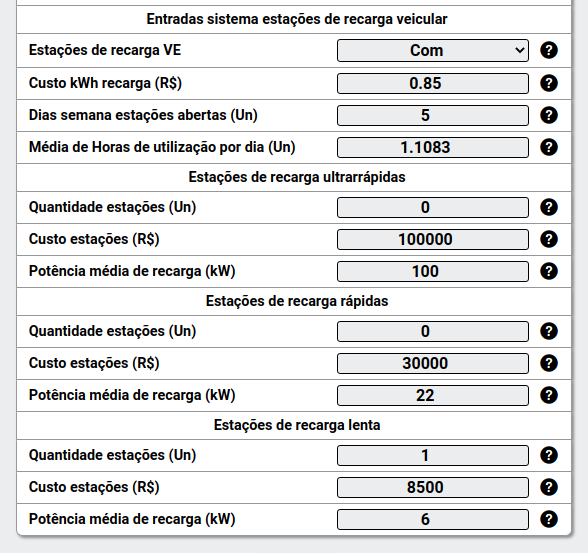
\includegraphics[width=1\textwidth]{./Figuras/casa_minha_2_3_2.png}
    \caption{Entradas para uma residência com telhado de 40 m² na cidade de Pelotas.}
   \label{fig:casa_minha_2_3_2}
\end{figure}

O resultado é mostrado na Figura \ref{fig:casa_minha_2_3}. Como esperado o sistema de estação de recarga não se paga, o faturamento bruto do sistema de recarga seria caso tivéssemos de pagar para a concessionária o custo de recarga deste veículo, nos resultado totais, a produção de energia é o suficiente para gerar um excedente de energia o suficiente para recarregar o veículo e pagar as taxas, o custo total do sistema aumenta devido a necessidade de mais painéis e a estação de recarga, o prazo de retorno do investimento sobe para 6 anos e 10 meses devido ao consumo extra, porém como este sistema tem durabilidade esperada de mais de 20 anos um pouco do custo acaba sendo amortizado ao longo dos anos pois o sistema gera um pequeno lucro.

\begin{figure}[H]
    \centering
    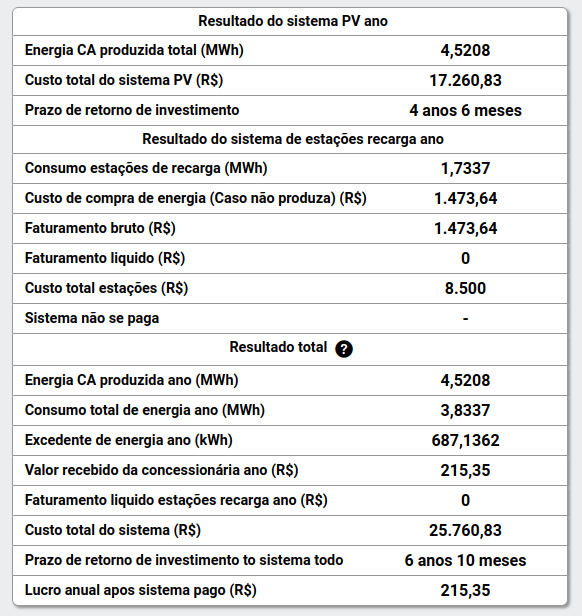
\includegraphics[width=1\textwidth]{./Figuras/casa_minha_2_3.png}
    \caption{Resultado para uma residência com telhado de 40 m² na cidade de Pelotas.}
   \label{fig:casa_minha_2_3}
\end{figure}
